\documentclass{article}
\usepackage[utf8]{inputenc}
\usepackage{subcaption}
\usepackage{graphicx}
\usepackage{placeins}
\usepackage{hyperref}

% Adjust these for the title of your report
% Your Student Name and Number.
\title{Assignment Title \& Example}
\author{SENG 474 Assignment \# \\Student Name \\ V00123456}
\date{February 2021}

\begin{document}

\maketitle

% Basic section header.
\section{Introduction}

% Adjust the large tags to adjust text size.
% The double \\ goes to next line.
\text{\large Example of Large text \\}
\text{\small Example of small}

% Example of a subsection.
\subsection{SubSection Example}\\
\text{\large Some equation examples to folow \\}

% Example equations.
\begin{equation}
    \alpha^X * C_0
\end{equation}
\\ \\

% Example of using math characters in text (\alpha, C_0)
\text{\large The values \(\alpha\) and \(C_0\) were fixed while X was incremented with each model starting at 0 and ending at 9.\\}

% This may cause an error if the Graphs Folder is not included.
% Example of a figure.
    \begin{figure}[h]
    % Adjust this line to change the image within the figure.
    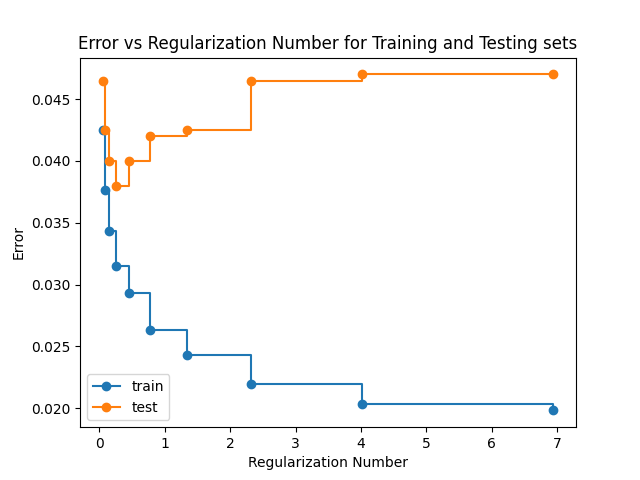
\includegraphics[width=1.0\linewidth, height=7.5cm]{Graphs/Unoptimized Logistic Regression.png} 
    \caption{Unoptimized Logistic Regression Error Results}
    \label{fig: Unotimized LR Results}
    \end{figure}

% Example of using the appoximate symbol.
\text{\large Looking at the actual error values at the closest point (Training: \(\approx\)4.25\%; Testing: \(\approx\)4.6\%) and the furthest point (Training: 2\%; Testing: \(\approx\)4.6\%) they only ever differ by a maximum of 2.6\%. Since the training error are small and relatively close to each other we can say this method produces best fit models.\\}

% Example of a table.
    \begin{table}[h!]
    \centering
    \begin{tabular}{|c | c | c |} 
     \hline
     Unoptimized (No KFold) & Error & Regularization Value\\
     \hline
    Training & 0.019833333333333335 & 6.940406893818192 \\ 
    \hline
     Testing & 0.038 & 0.25888585 \\
     \hline
    \end{tabular}
    \caption{Best Unoptimized Logistic Regression Errors.}
    \label{table:1}
    \end{table}

% Example of using the plus/minus symbol.
\text{\large Using Z as 1.96, I calculated the following confidence interval 3.8\% \(\pm\) 0.8\%. Meaning the true testing error is between 3.0\% and 4.6\%.}

% This Float barrier tag prevents figures from appearing past this point, in this case, the next section.
\FloatBarrier

\section{Split Table Example}

    \begin{table}[h!]
    \centering
    \begin{tabular}{|c | c | c |} 
    \hline
    Unoptimized (No KFold) & Error & Regularization Value\\
    \hline
    Training & 0.019833333333333335 & 6.940406893818192 \\ 
    \hline
    Testing & 0.038 & 0.25888585 \\
    \hline\hline
    Optimized (KFold) & Error & Regularization Value\\
    \hline
    Training & 0.024166666666666666 & 1.4361450195312502 \\ 
    \hline
     Testing & 0.043 & 1.4361450195312502 \\
     \hline
    \end{tabular}
    \caption{Best Unoptimized \& Optimized Logistic Regression Errors.}
    \label{table:3}
    \end{table}
 
\section{References (IEEE Examples)}
\text{[1] \textit{"RBF SVM parameters"}, Scikit-learn, Accessed on: Feb 27, 2021.[Online]. Available: \url{https://scikit-learn.org/stable/auto_examples/svm/plot_rbf_parameters.html} \\ \\}
\end{document}
